% experiments.tex

\section{Experiments}

\begin{figure}[t]
\centering
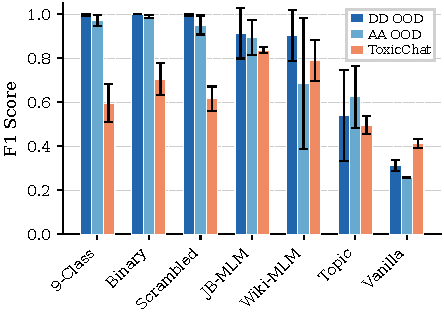
\includegraphics[width=\columnwidth]{figures/paper/fig3_evidence_hierarchy.pdf}
\caption{Evidence hierarchy across evaluation conditions. Classification-based DAPT outperforms MLM and vanilla on synthetic OOD attacks (DD, AA), but the hierarchy reverses on human-authored single-turn data (ToxicChat), where JB-MLM leads.}
\label{fig:evidence_hierarchy}
\end{figure}

\paragraph{Terminology.}
\emph{Cross-attack OOD}: evaluation on attack families unseen during training; benign distribution remains in-distribution (IID) throughout (OOD reflects attack-side shift only). $K$: prefix length (number of conversation turns retained). \emph{DAPT}: all Stage-1 adaptations; we extend \citet{gururangan2020dontstop} to supervised variants. We refer to the performance ranking of DAPT variants across OOD conditions as the \emph{evidence hierarchy} (Section~\ref{sec:decomposition}).

\begin{table}[t]
\centering
\small
\caption{Cross-attack generalization (F1) at $K$=2 and full conversation length. IID: Crescendo; OOD: Deceptive Delight (DD). 3-seed mean$\pm$std where noted; full per-$K$ in Appendix~\ref{sec:full_prefix}.}
\label{tab:main_results}
\resizebox{\columnwidth}{!}{%
\begin{tabular}{@{}lcc|cc@{}}
\toprule
& \multicolumn{2}{c|}{\textit{IID (Cresc.)}} & \multicolumn{2}{c}{\textit{OOD (DD)}} \\
\textbf{Method} & $K$=2 & Full & $K$=2 & Full \\
\midrule
9-class & \textbf{1.000$\pm$.000} & \textbf{1.000$\pm$.000} & .981$\pm$.013 & \textbf{.997$\pm$.005} \\
MLM-only$^{\ddagger}$ & .974 & 1.000 & \textbf{.993$\pm$.009} & .914$\pm$.115 \\
Vanilla & .978$\pm$.016 & 1.000$\pm$.000 & .479$\pm$.038 & .312$\pm$.026 \\
TF-IDF LR$^{\S}$ & 1.000 & 1.000 & 1.000 & .961 \\
\bottomrule
\end{tabular}}
\vspace{-2pt}
{\footnotesize $^{\ddagger}$MLM-only IID reports single seed (42); OOD reports 3-seed. $^{\S}$TF-IDF is deterministic (no std).}
\end{table}

\subsection{Setup}

\paragraph{Data.}
All synthetic data is generated by Qwen3-8B~\citep{qwen3_2025}.
The IID dataset contains 250 Crescendo~\citep{russinovich2024crescendo} jailbreak and 250 benign conversations, split into training (350), validation (74), and test (76) with balanced classes.
Stage~1 uses training + validation; Stage~2 trains on training, early-stops on validation.
OOD evaluation pairs 80 attack-specific conversations with 38 IID-test benign: FITD~\citep{fitd2024}, DD~\citep{deceptivedelight2024}, and ActorAttack~\citep{ren2024actorattack} (118 total each; no template overlap across families).
A paraphrased IID test set (BERTScore 0.92) serves as the robustness benchmark (Section~\ref{sec:perturbation}).
For human validation, we use ToxicChat~\citep{lin2023toxicchat} (204+204 from real LMSYS interactions).

\paragraph{Models.}
Seven DeBERTa-v3 variants share the same Stage-2 pipeline and differ only in Stage-1 training (Section~\ref{sec:method}).
Our vanilla DeBERTa+BiGRU configuration is architecturally equivalent to DeepContext~\citep{deepcontext2026} and differs only in encoder choice (DeBERTa-v3-base vs.\ BERT); it serves as our primary baseline.
For cross-encoder validation, we replicate vanilla, MLM, and 9-class variants on RoBERTa-base~\citep{liu2019roberta} (Section~\ref{sec:cross_encoder}).
We also compare TF-IDF (term frequency--inverse document frequency) logistic regression, LLM-as-judge (Appendix~\ref{sec:llm_judge}), and Llama Guard~3~8B~\citep{metallamaguard3_2024} (zero-shot; evaluates last-response safety given conversation context), which detects only 1.8\% of multi-turn jailbreaks (5/278 pooled recall; Table~\ref{tab:evidence_hierarchy}).

\paragraph{Metrics.}
F1 for binary jailbreak detection at prefix $K$=2 and full conversations (full per-$K$ in Appendix~\ref{sec:full_prefix}).
OOD results report 3-seed mean$\pm$std (seeds 42, 123, 456).
For pairwise comparisons, we report bias-corrected and accelerated (BCa) bootstrap 95\% confidence intervals (10,000 resamples; assumes cross-seed independence) and paired permutation tests; seed-level values confirm all conclusions hold at every seed (Appendix~\ref{app:seed_level}).

\paragraph{Training.}
Stage-1: learning rate $2 \times 10^{-5}$, batch 16, 4 epochs, MLM masking 15\%.
Stage-2: two-layer MLP, 20 epochs.

%----------------------------------------------------------------------
\subsection{Cross-Attack Generalization}

Vanilla encoders collapse under cross-attack transfer; domain-adapted variants recover near-perfect detection (Table~\ref{tab:main_results}, Figure~\ref{fig:cross_attack_bar}).
On OOD DD, vanilla drops to F1\,=\,0.312$\pm$0.026 and worsens with more turns (0.628$\to$0.312 at Full), consistent with attack turns occupying benign embedding regions~\citep{bullwinkel2025repeng}. MLM recovers to $\geq$0.97 at $K \leq 5$ without labels but is unstable at full length (0.914$\pm$0.115); 9-class maintains 0.997$\pm$0.005.
On strategy-diverse ActorAttack, TF-IDF collapses (0.261) while 9-class maintains 0.972$\pm$0.026, a 71 percentage point (pp) gap that confirms domain-adapted representations capture beyond-lexical features.
Seed-level results confirm consistent separation (Table~\ref{tab:seed_level}; bootstrap CIs non-overlapping, permutation $p < 0.0001$). FITD is non-discriminative (all F1\,$\geq$\,0.990).

\begin{figure}[t]
\centering
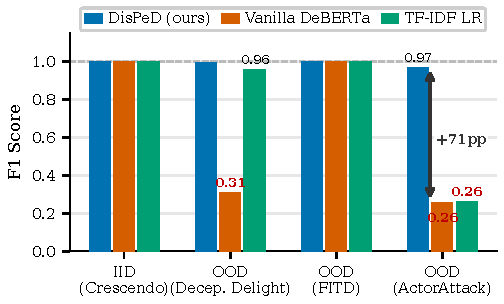
\includegraphics[width=\columnwidth]{figures/paper/fig2_cross_attack_bar.pdf}
\caption{Cross-attack overview (F1 at full conversation length). DisPeD (9-class) maintains near-perfect detection across IID and both OOD families; vanilla collapses on OOD DD. FITD is non-discriminative for all methods.}
\label{fig:cross_attack_bar}
\end{figure}

Prefix-length analysis (Appendix Table~\ref{tab:full_prefix}) confirms 9-class stability across all prefixes (0.972--0.997) vs.\ MLM instability at full length (0.914$\pm$0.115) and vanilla degradation (0.628$\to$0.312).

%----------------------------------------------------------------------
\subsection{Decomposing the Detection Mechanism}
\label{sec:decomposition}

\begin{table}[t]
\centering
\small
\caption{Evidence hierarchy on OOD DD and ActorAttack (AA) at full conversation length (3-seed mean$\pm$std where available). OOD F1 reflects attack-side generalization only; benign samples are IID from training distribution (benign-side shift evaluated in Section~\ref{sec:benign_shift}). Bold indicates best per column. All variants share the same Stage-2 pipeline. Full per-prefix results in Appendix Tables~\ref{tab:full_prefix} and~\ref{tab:actorattack_full}. Bottom rows: full dual-OOD evaluation with WildChat benign replacing IID benign (Appendix~\ref{app:dual_ood}).}
\label{tab:evidence_hierarchy}
\resizebox{\columnwidth}{!}{%
\begin{tabular}{@{}lccc@{}}
\toprule
\textbf{Variant} & DD-Full & AA-Full & DD-$K$=2 \\
\midrule
9-class (full model) & .997$\pm$.005 & .972$\pm$.026 & .981$\pm$.013 \\
Binary (2-class) & \textbf{1.000$\pm$.000} & \textbf{.990$\pm$.008} & .994$\pm$.009 \\
Scrambled labels & .997$\pm$.005 & .951$\pm$.043 & .981$\pm$.026 \\
MLM-only$^{\ddagger}$ (no labels) & .914$\pm$.115 & .893$\pm$.080 & .993$\pm$.009 \\
Mean pooling$^{*}$ & .991$\pm$.013 & .962$\pm$.015 & .994$\pm$.009 \\
\midrule
Topic classif.\ (5-class) & .541$\pm$.207 & .625$\pm$.141 & .593$\pm$.166 \\
Wikipedia MLM & .904$\pm$.115 & .686$\pm$.297 & .911$\pm$.073 \\
Vanilla DeBERTa & .312$\pm$.026 & .258$\pm$.000 & .479$\pm$.038 \\
TF-IDF LR$^{\dagger}$ & .961 & .261 & \textbf{1.000} \\
Llama Guard~3$^{\P}$ & .024 & .000 & -- \\
\midrule
\multicolumn{4}{l}{\textit{Dual-OOD (WildChat benign; Section~\ref{sec:benign_shift})}} \\[2pt]
9-class (no adapt) & .855 & .842 & -- \\
9-class (+10-shot) & .994 & .981 & -- \\
\bottomrule
\end{tabular}}
\vspace{-2pt}
{\footnotesize $^{*}$9-class encoder with mean pooling replacing BiGRU. $^{\dagger}$Deterministic (no std). $^{\ddagger}$MLM-only IID (Table~\ref{tab:main_results}) is single-seed (42); all OOD values are 3-seed. $^{\P}$Zero-shot; no domain training.}
\end{table}

A clear \emph{evidence hierarchy} emerges across seven variants on synthetic multi-turn data (Table~\ref{tab:evidence_hierarchy}, Figure~\ref{fig:evidence_hierarchy}), ordered by OOD detection at full conversation length: vanilla $<$ topic $\ll$ MLM $<$ classification-supervised ($\approx$\,1.0 on DD).

\paragraph{Domain exposure is the primary observed factor.}
MLM bridges $\sim$60\,pp from vanilla (0.312$\pm$0.026 $\to$ 0.914$\pm$0.115) without labels; this supports the DAPT interpretation~\citep{gururangan2020dontstop}. TF-IDF collapse on ActorAttack (0.261 vs.\ 9-class 0.972) confirms that domain-adapted representations capture features beyond lexical overlap.
All three classification-supervised variants converge to equivalent detection (F1 = 0.997--1.000); McNemar's ($p > 0.13$) and paired permutation tests ($p \geq 0.40$) provide descriptive evidence suggesting equivalence. Extended to $n$\,=\,10 seeds, TOST (margin = 5\,pp) confirms equivalence on DD ($p < 10^{-8}$, $d$\,=\,$-$0.14; Table~\ref{tab:tost_sensitivity}) and FITD ($p < 10^{-8}$, $d \approx 0$). Label quality and granularity are non-factors for template-attack detection (DD/FITD: $|d| \leq 0.14$), but strategy-diverse ActorAttack retains moderate label sensitivity ($d$\,=\,0.44, TOST $p$\,=\,0.183). For template attacks, any domain-relevant classification objective suffices; the structural role of the objective (partitioning the representation space) matters more than label semantics. Strategy-diverse attacks mark a difficulty boundary for this sufficiency.
Classification supervision is associated with 3--23$\times$ lower cross-seed variance over MLM on synthetic OOD (std 0.005 vs.\ 0.115 on DD; 3 seeds; Appendix~\ref{app:ensemble}), though this reverses on human-authored data (Section~\ref{sec:human_data}).

\begin{table}[t]
\centering
\footnotesize
\caption{Cross-encoder comparison on OOD Full (3-seed mean$\pm$std). DD = Deceptive Delight, AA = ActorAttack. Bold indicates best per encoder group.}
\label{tab:cross_encoder}
\begin{tabular}{@{}lcc@{}}
\toprule
\textbf{Variant} & DD & AA \\
\midrule
\multicolumn{3}{l}{\textit{DeBERTa-v3-base (184M)}} \\[2pt]
Vanilla & .312$\pm$.026 & .258$\pm$.000 \\
MLM & .914$\pm$.115 & .893$\pm$.080 \\
9-class & \textbf{.997$\pm$.005} & \textbf{.972$\pm$.026} \\
\midrule
\multicolumn{3}{l}{\textit{RoBERTa-base (125M)}} \\[2pt]
Vanilla & .981$\pm$.026 & .466$\pm$.163 \\
MLM & .987$\pm$.018 & .730$\pm$.201 \\
9-class & \textbf{.994$\pm$.005} & \textbf{.939$\pm$.046} \\
\midrule
\multicolumn{3}{l}{\textit{RoBERTa-large (355M)}} \\[2pt]
Vanilla & .927$\pm$.036 & \textbf{1.000$\pm$.000} \\
MLM & .884$\pm$.065 & .874$\pm$.014 \\
9-class & \textbf{.987$\pm$.004} & .946$\pm$.057 \\
\bottomrule
\end{tabular}
\end{table}

\paragraph{Domain specificity is marginal at full length but meaningful for early detection.}
Wikipedia MLM (0.904$\pm$0.115) nearly matches jailbreak-domain MLM at full length (1\,pp gap), though jailbreak-domain text provides an 8\,pp advantage at early prefixes ($K$=2: 0.993 vs.\ 0.911).
Perturbation analysis (Section~\ref{sec:perturbation}) reveals a sharper domain specificity effect: Wikipedia MLM degrades by $\sim$12\,pp under adversarial paraphrasing while jailbreak-domain MLM degrades by only 2.6\,pp.

\paragraph{Misaligned supervision destabilizes generalization.}
Topic classification's poor performance (0.541$\pm$0.207) is consistent with misaligned supervision; the cleaner test isolating domain exposure is Wiki-MLM vs.\ JB-MLM (Section~\ref{sec:decomposition}).

\paragraph{Evidence hierarchy on strategy-diverse attacks.}
ActorAttack~\citep{ren2024actorattack} preserves the same hierarchy (Figure~\ref{fig:evidence_hierarchy}) with wider gaps: TF-IDF collapses (0.261) while classification variants converge (0.951--0.990, max gap 3.9\,pp); DAPT provides $\sim$71\,pp over vanilla (Appendix~\ref{sec:actorattack_full},~\ref{app:aa_error}).

\paragraph{Temporal modeling.}
Mean pooling matches BiGRU (F1 gap $\leq$ 1\,pp; Appendix~\ref{app:temporal}) and turn-order shuffling is negligible ($|\Delta| < 1$\,pp); detection therefore relies on per-turn content rather than sequential patterns.

%----------------------------------------------------------------------
\subsection{Cross-Encoder Validation}
\label{sec:cross_encoder}

To test whether the evidence hierarchy depends on encoder choice, we replicate vanilla, MLM, and 9-class on RoBERTa-base~\citep{liu2019roberta} (Table~\ref{tab:cross_encoder}).
On DD, RoBERTa-base vanilla already achieves 0.981$\pm$0.026 (vs.\ DeBERTa 0.312$\pm$0.026), so DAPT adds only 1.3\,pp. ActorAttack exposes this as DD's simplicity: RoBERTa-base vanilla collapses to 0.466$\pm$0.163, a 51.5\,pp drop, while domain-adapted variants recover (9-class: 0.939$\pm$0.046).

RoBERTa-large (355M) reverses the DAPT advantage on ActorAttack (vanilla 1.000 vs.\ 9-class 0.946; Table~\ref{tab:roberta_large_lr}). This exposes a difficulty threshold: base-scale encoders require DAPT for all attacks, while sufficient capacity renders it unnecessary. A BERT-base proxy confirms DAPT, not architecture, drives generalization (Appendix~\ref{app:bert_proxy}).

\begin{figure}[t]
\centering
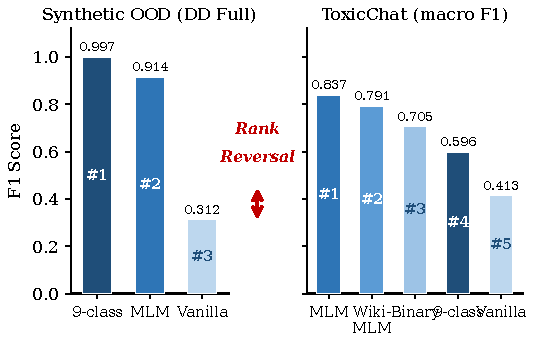
\includegraphics[width=\columnwidth]{figures/paper/fig_hierarchy_reversal.pdf}
\caption{Condition-specific evidence hierarchy. On synthetic OOD (DD), classification DAPT dominates; on human-authored ToxicChat, unsupervised MLM leads, and rank positions reverse entirely.}
\label{fig:hierarchy_reversal}
\end{figure}

%----------------------------------------------------------------------
\subsection{Mixed-LLM Training}

All preceding experiments use single-source (Qwen3-8B) data. To test whether the evidence hierarchy transfers when training data mixes LLM sources, we train on 250 Qwen + 250 Llama-3.1-8B conversations (Table~\ref{tab:mixed_llm}).
Classification-based DAPT is the only variant that substantially outperforms vanilla: 9-class achieves DD OOD F1\,=\,0.818$\pm$0.096 (+53\,pp over vanilla 0.291$\pm$0.065), while MLM drops to vanilla level (0.289$\pm$0.101). On strategy-diverse ActorAttack, detection degrades to chance level (9-class F1\,=\,0.504$\pm$0.107, indistinguishable from majority baseline at $n$\,=\,3).
Classification supervision thus generalizes across LLM sources where unsupervised pretraining does not (Appendix~\ref{app:mixed_llm}).

%----------------------------------------------------------------------
\subsection{Human Data Validation}
\label{sec:human_data}

Since both training and OOD evaluation data are Qwen3-8B-generated, we validate on ToxicChat~\citep{lin2023toxicchat} (204 human-written jailbreak attempts + 204 benign conversations from real LMSYS interactions).

\begin{table}[t]
\centering
\small
\caption{Human data validation on ToxicChat~\citep{lin2023toxicchat} (macro F1, 3-seed mean$\pm$std). Bold indicates best. Single-turn data from real LMSYS user interactions, independent of Qwen3-8B.}
\label{tab:human_data}
\begin{tabular}{@{}lc@{}}
\toprule
\textbf{Variant} & Macro F1 \\
\midrule
JB-MLM & \textbf{.837$\pm$.013} \\
Wiki-MLM & .791$\pm$.093 \\
Binary & .705$\pm$.072 \\
Scrambled & .616$\pm$.056 \\
9-class & .596$\pm$.087 \\
Topic & .496$\pm$.042 \\
\midrule
Vanilla & .413$\pm$.021 \\
\bottomrule
\end{tabular}
\end{table}

The ordering reverses (Table~\ref{tab:human_data}; Figure~\ref{fig:hierarchy_reversal}): JB-MLM leads (0.837$\pm$0.013) while 9-class ranks lower (0.596$\pm$0.087; $p < 0.001$). All jailbreak-domain DAPT variants exceed vanilla by 18--42\,pp, which confirms transfer to human-written attacks. ToxicChat is single-turn, so the classification head provides no advantage.

%----------------------------------------------------------------------
\subsection{Robustness and Strategy Analysis}
\label{sec:perturbation}

Under adversarial paraphrasing (BERTScore 0.92), classification variants achieve zero degradation on OOD DD while non-adapted models degrade by $\sim$12\,pp; on ActorAttack, DAPT degrades ($\Delta$\,=\,$-$20.4\,pp) but maintains 52\,pp over vanilla (Table~\ref{tab:ood_perturbation}; Appendices~\ref{sec:perturbation_full},~\ref{sec:strategy_full}). The 9-class taxonomy characterizes known attacks ($\kappa$\,=\,0.78) but degrades on OOD ($\kappa$\,=\,0.126; Appendix~\ref{app:strategy_pred}); detection operates through \texttt{[CLS]} embeddings, not strategy accuracy.

%----------------------------------------------------------------------
\subsection{Benign Distribution Shift}
\label{sec:benign_shift}

\begin{figure}[t]
\centering
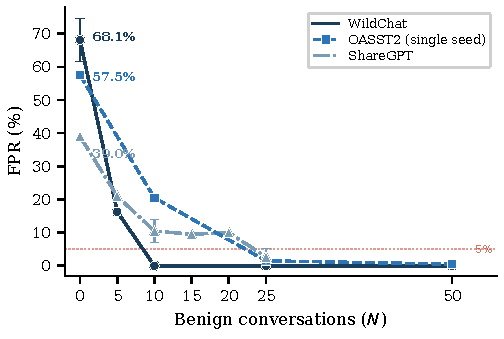
\includegraphics[width=\columnwidth]{figures/paper/fig_fpr_adaptation.pdf}
\caption{Few-shot benign adaptation reduces FPR below the 5\% deployment threshold with 10--25 conversations across three platforms.}
\label{fig:fpr_adaptation}
\end{figure}

On WildChat benign conversations, 9-class FPR rises to 68.1\% (Appendix~\ref{app:wildchat_fpr}). Few-shot adaptation (encoder frozen, $N$ benign conversations) resolves this (Figure~\ref{fig:fpr_adaptation}): 10 WildChat conversations reduce FPR to 0\%, 25 OASST2 to 1.5\% (consistent across WildChat, OASST2, and ShareGPT; Appendix~\ref{app:oasst2}); dual-OOD F1 drops 13--14\,pp without adaptation but recovers within 0.3\,pp (Appendix~\ref{app:dual_ood}).
